\documentclass[11pt,a4paper,DIV=12]{scrartcl}

% Pakete einbinden, die benötigt werden
\usepackage{scrlayer-scrpage}
\usepackage[utf8]{inputenc}       % Dateien in UTF-8 benutzen
\usepackage[T1]{fontenc}          % Zeichenkodierung
\usepackage{graphicx}             % Bilder einbinden
\usepackage[main=ngerman, english]{babel}  % Deutsche Sprachunterstützung
\usepackage[autostyle=true,german=quotes]{csquotes} % Deutsche Anführungszeichen
\usepackage[pagebackref=false,german]{hyperref} % Hyperlinks
\usepackage{xcolor}               % Unterstützung für Farben
\usepackage{amsmath}              % Mathematische Formeln
\usepackage{amsfonts}             % Mathematische Zeichensätze
\usepackage{amssymb}              % Mathematische Symbole
\usepackage{float}                % Fließende Objekte (Tabellen, Grafiken etc.)
\usepackage{booktabs}             % Korrekter Tabellensatz
\usepackage{listings}             % Quelltexte
\usepackage{listingsutf8}         % Quelltexte in UTF8
\usepackage[hang,font={sf,footnotesize},labelfont={footnotesize,bf}]{caption} % Beschriftungen
\usepackage[scaled]{helvet}       % Schrift Helvetia laden
\usepackage[bottom=25mm,left=30mm,right=30mm,top=25mm]{geometry} % Ränder ändern
\usepackage{setspace}             % Abstände korrigieren
\usepackage{scrhack}              % tocbasic Warnung entfernen
\usepackage[all]{hypcap}          % Korrekte Verlinkung von Floats
\usepackage{tabularx}             % Spezielle Tabellen
\usepackage{rotating}             % Seiten drehen
\usepackage{array}

 % Einstellungen für Schriftarten
\setkomafont{titlehead}{\centering\normalfont\sffamily}
\setkomafont{author}{\normalfont\sffamily}
\setkomafont{publishers}{\normalfont\sffamily}
\setkomafont{date}{\normalfont\sffamily}
\setkomafont{title}{\normalfont\sffamily\bfseries\LARGE}
\setkomafont{pagehead}{\normalfont\sffamily}
\setkomafont{pagenumber}{\normalfont\sffamily}
\setkomafont{paragraph}{\sffamily\bfseries\small}
\setkomafont{subsection}{\sffamily\bfseries\Large}
\setkomafont{subsubsection}{\sffamily\itshape\bfseries\small}
\addtokomafont{footnote}{\footnotesize}

% Wichtige Abstände
\setlength{\parskip}{0.2cm}  % 2mm Abstand zwischen zwei Absätzen
\setlength{\parindent}{0mm}  % Absätze nicht einziehen
\clubpenalty = 10000         % Keine "Schusterjungen"
\widowpenalty = 10000        % Keine "Hurenkinder"
\displaywidowpenalty = 10000 % Keine "Hurenkinder"
                             % Siehe: https://de.wikipedia.org/wiki/Hurenkind_und_Schusterjunge

% Einfacher Font-Wechsel über dieses Makro
\newcommand{\changefont}[3]{
\fontfamily{#1} \fontseries{#2} \fontshape{#3} \selectfont}

\changefont{ptm}{m}{n}  % Times New Roman für den Fließtext
\renewcommand{\rmdefault}{ptm}

\newcommand{\loesung}{\textbf{Lösung:}\\}

\newcommand{\abgabetermin}[1]{\publishers{\textbf{Abgabetermin: #1}}}

\newcommand{\kapitel}[1]{\setcounter{section}{#1}}

\newcommand{\kapitelname}[1]{\title{Übungsblatt \thesection: #1}}

\newcolumntype{L}{>{\raggedright\arraybackslash}X}

\RedeclareSectionCommand[
  beforeskip=-1.0\baselineskip,
  afterskip=0.01\baselineskip]{section}

\RedeclareSectionCommand[
  beforeskip=-1.0\baselineskip,
  afterskip=0.01\baselineskip]{subsection}

\titlehead{Einführung in die Informatik (EI) -- Prof. Thomas Smits -- Wintersemester 2019/2020}

\date{\today}

%%%%%%%%%%%%%%%%%%%%%%%%%%%%%%%%%%%%%%%%%%%%%%%%%%%%%%%%%%%%%%%%%%%%%%%%%%%%%%
% Hier beginnt das eigentliche Dokument
% An den Einstellungen davor müssen Sie normalerweise keine Änderungen
% vornehmen.
%%%%%%%%%%%%%%%%%%%%%%%%%%%%%%%%%%%%%%%%%%%%%%%%%%%%%%%%%%%%%%%%%%%%%%%%%%%%%%

% Bitte tragen Sie hier Ihren Namen und Ihre Mattrikelnummer ein
\author{Peter Mustermann\\ (1992822)}

% Welches Übungsblatt zu welchem Thema bearbeiten Sie?
\kapitel{1}
\kapitelname{Einführung}

\begin{document} % Hier beginnt das eigentliche Dokument
\maketitle       % Titel erzeugen

% ----------------------------------------------------------------------------
% Jede Aufgabe bekommt eine subsection. Die Nummerierung erfolgt automatisch
\subsection{Herkunft der Informatik}

% Sinnvollerweise wiederholen Sie die Frage noch einmal
Aus welchen Wissenschaften ist die Informatik in erster Linie hervorgegangen?

% Hier beginnt Ihre Lösung
\loesung
Historisch gesehen ist die Informatik in erster Linie aus der Mathematik und der Elektrotechnik hervorgegangen. Von Bedeutung sind daneben auch andere Ingenieurwissenschaften, außerdem Physik (insbesondere die Festkörperphysik), Linguistik und BWL sowie zahlreiche Disziplinen in speziellen Anwendungen, beispielsweise Medizin, Biologie und Medientechnik.

% ----------------------------------------------------------------------------
\subsection{Definition Informatik}
Finden Sie eine oder mehrere Definitionen des Begriffs \emph{Informatik} und geben Sie diese wieder.

\loesung
\enquote{Informatik ist die Wissenschaft der systematischen Verarbeitung und
Übermittlung von Informationen unter Verwendung von
programmierbareren Digitalrechnern.} (G. Büchel, Praktische Informatik)

\enquote{Informatik = Information und Automatik; Wissenschaft rund um die systematische Verarbeitung und Speicherung von Informationen.} (Fischer Lexikon der Informatik)

% ----------------------------------------------------------------------------
\subsection{Definition Digitalrechner}
Finden Sie eine Definition des Begriffs \emph{Digitalrechner} und geben Sie diese wieder.

\loesung
\enquote{Ein Digitalrechner ist ein Rechner, der seine Informationen intern durch Ziffern (digits) darstellt, wobei die Zifferndarstellung von definierten Spannungszuständen abhängt. Das Ziffernalphabet der vorherrschenden Digitalrechner besteht aus den Ziffern 0 und 1.} (G. Büchel, Praktische Informatik)

% ----------------------------------------------------------------------------
\subsection{Themenbereiche der Informatik}
Geben Sie jeweils ein Beispiel für Themen, mit denen sich die verschiedenen Gebiete der Informatik (Technische, Theoretische, Praktische, Angewandte) beschäftigen.

Geben Sie zu jedem Thema mit ein paar Stichpunkten an, worum es sich handelt.

\loesung
Definitionen entnommen dem Fischer Lexikon der Informatik
\newline

\begin{tabularx}{\textwidth}{l L L}
\toprule
\textbf{Gebiet} & \textbf{Definition} & \textbf{Beispiel}\\
\midrule
\emph{Praktische Informatik} & Informatik-Disziplinen, welche sich vorwiegend mit der Entwicklung und Anwendung der Software-Komponenten befassen & Programmentwicklung, Compilerbau; im Aufbau von z.B. Informationssystemen und Netzwerken ergeben sich Überlappungen mit der technischen Informatik \\
\emph{Technische Informatik} & Informatik-Disziplinen, welche sich vorwiegend mit der Entwicklung und Anwendung der Hardware-Komponenten befassen & Digitaltechnik, Mikroprozessortechnik \\
\emph{Theoretische Informatik} & Informatik-Disziplinen, welche sich mit der Entwicklung von Theorien und Modellen der Informatik befassen und dabei viel Substanz aus der Mathematik konsumieren & Relationenmodell, Objekt-Paradigmen, Komplexitätstheorie, Kalküle \\
\emph{Angewandte Informatik} & Informatik als instrumentale Wissenschaft & Rechtsinformatik, Wirtschaftsinformatik, Geoinformatik \\
\bottomrule
\end{tabularx}

% ----------------------------------------------------------------------------
\subsection{Erster Digitalrechner (Computer)}
Welchen Rechner/welche Rechner kann man als ersten universell und frei programmierbaren Computer betrachten?

\loesung
Beim ersten Computer, der frei und universell programmierbar war, handelte es sich um die Zuse Z3. Diese wurde 1941 von Konrad Zuse in Zusammenarbeit mit Helmut Schreyer in Berlin gebaut. Die Z3 wurde in elektromagnetischer Relaistechnik mit 600 Relais für das Rechenwerk und 1400 Relais für das Speicherwerk ausgeführt. Da die Z3 aber nicht freiprogrammierbar genutzt wurde und im zweiten Weltkrieg zerstört, wird oft ein anderer Rechner genannt: Der Harvard Mark I.

Der Harvard Mark I, auch Automatic Sequence Controlled Calculator (ASCC) genannt, ist ein in den USA zwischen 1943 und 1944 vollständig aus elektromechanischen Bauteilen von Howard H. Aiken gebauter früher Computer.

\begin{figure}[ht!]
  \centering
  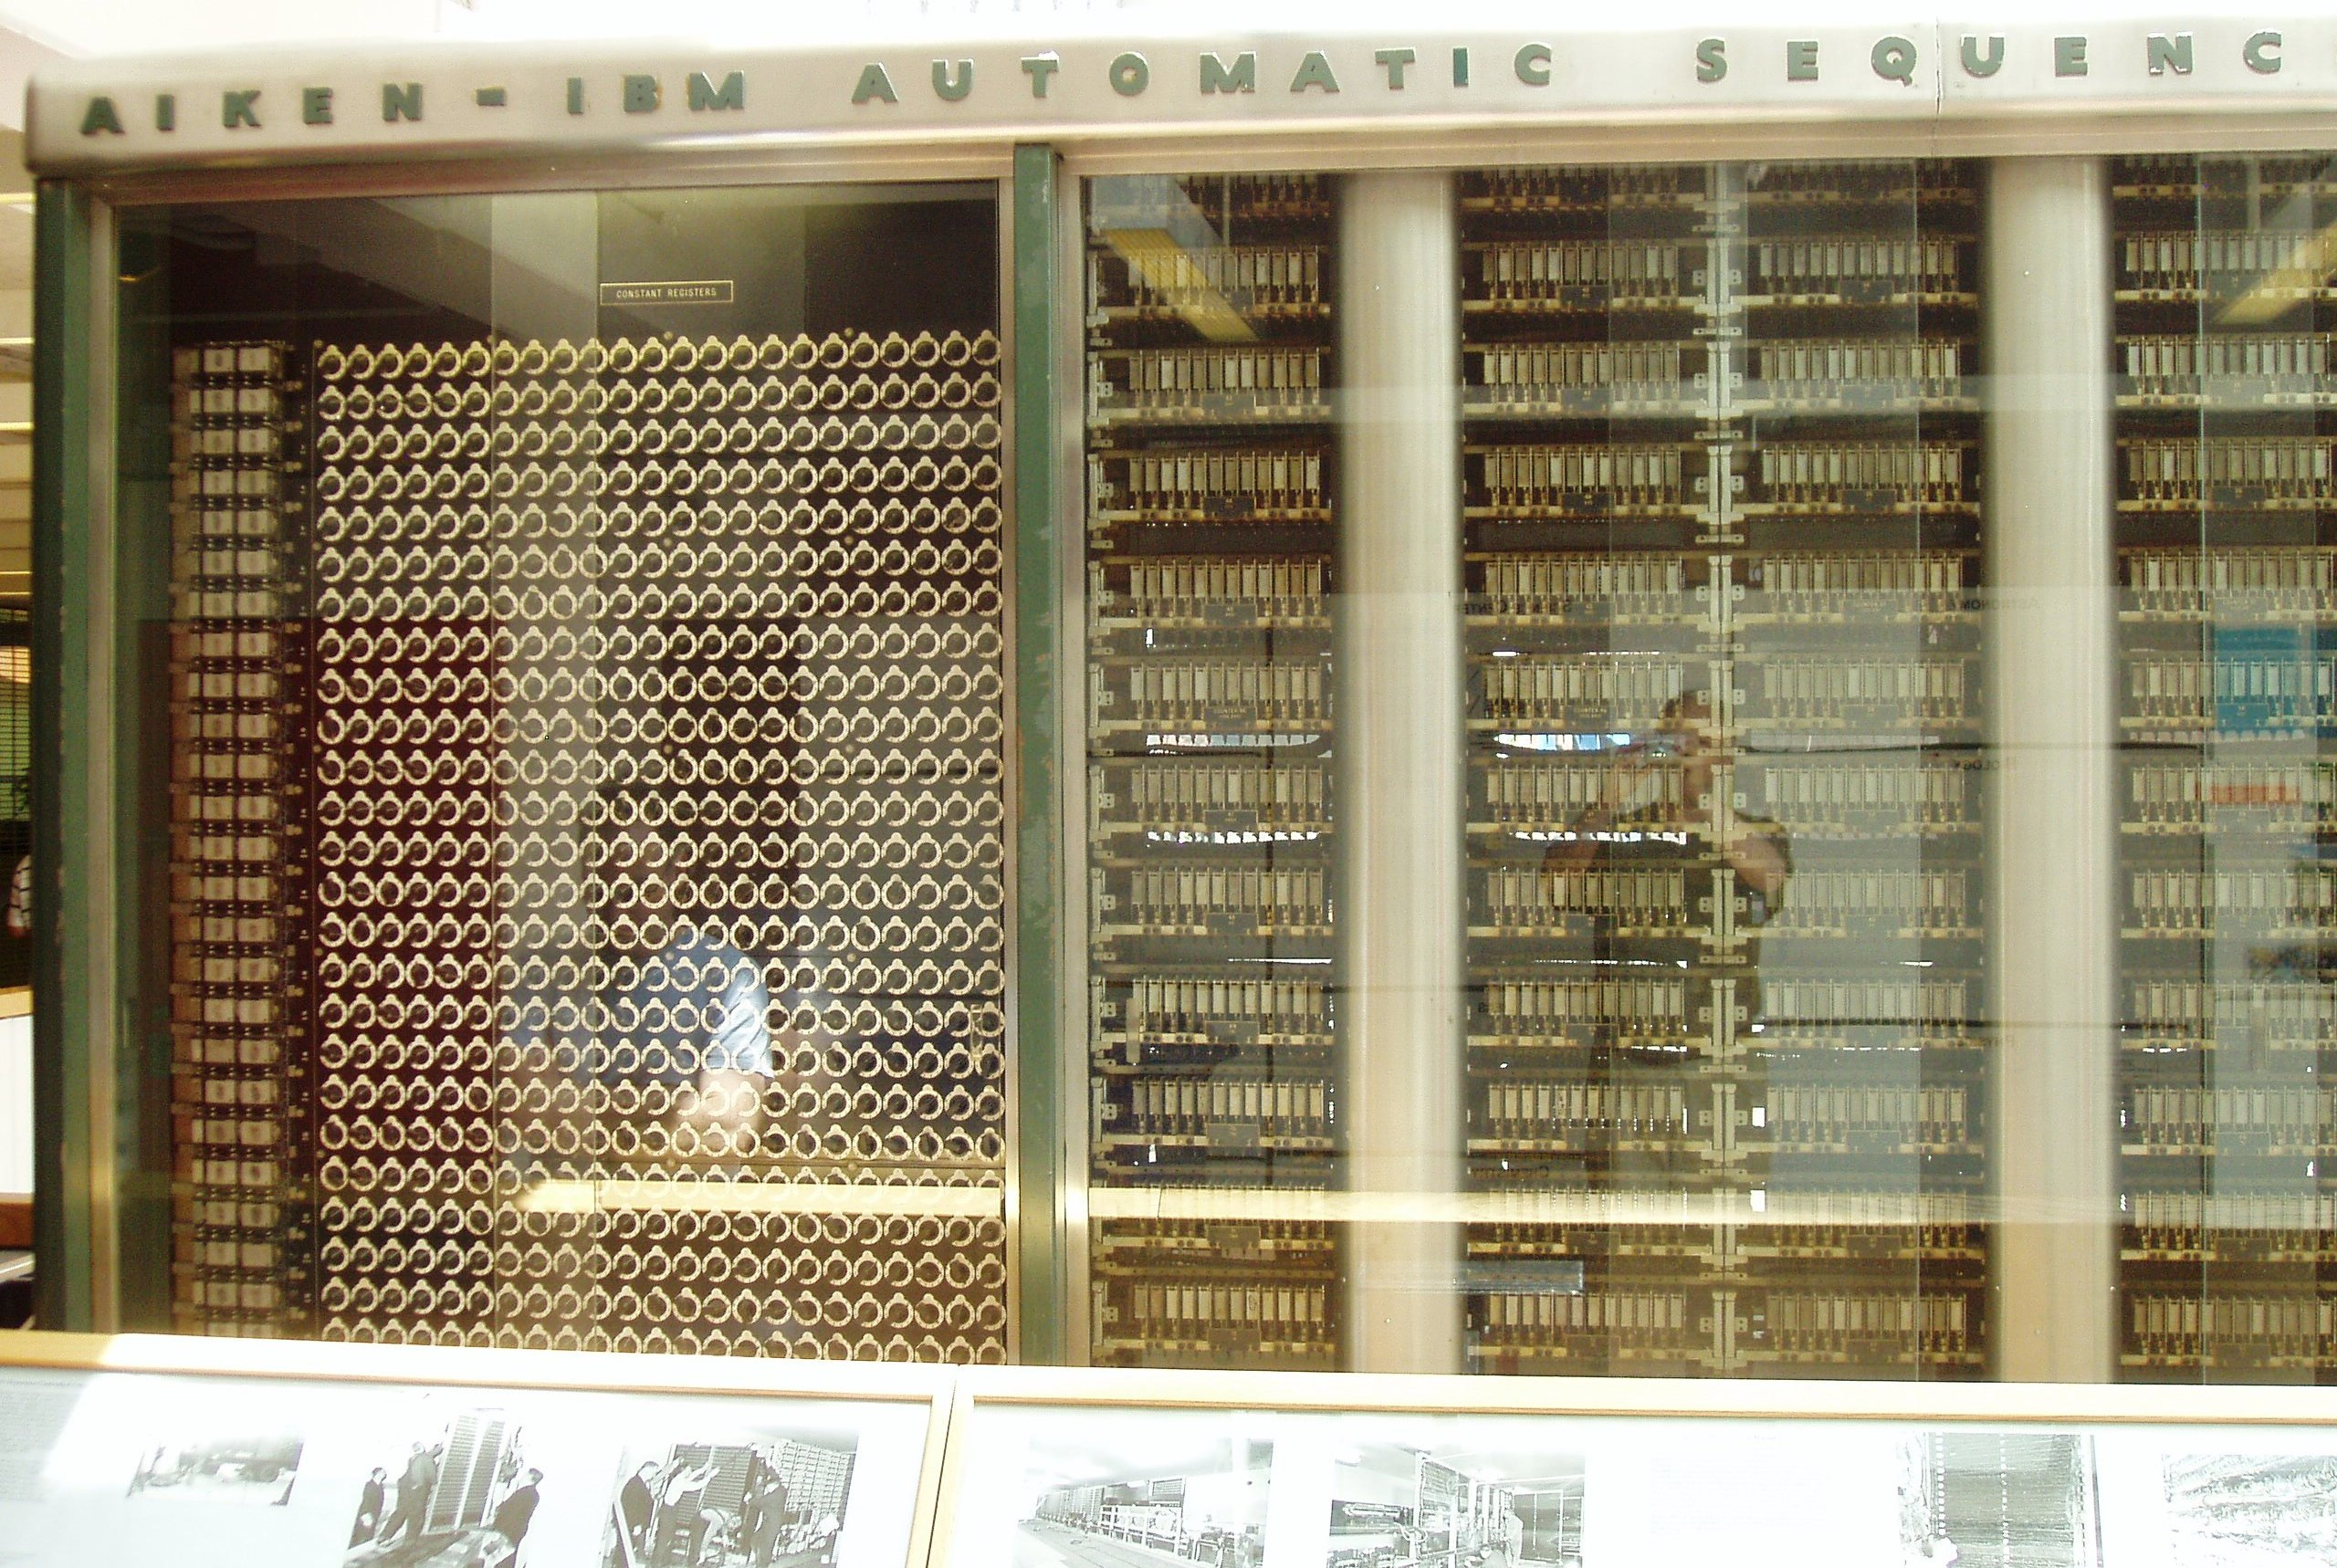
\includegraphics[width=7cm]{img/mark_i_wikipedia.jpg}
  \caption{Mark I}
\end{figure}

% ----------------------------------------------------------------------------
\subsection{Konrad Zuse}
Welche Bedeutung kommt Konrad Zuse für die Informatik zu? Warum wird sein Beitrag häufig übersehen?

\loesung
Konrad Ernst Otto Zuse war ein deutscher Bauingenieur, Erfinder und Unternehmer. Mit seiner Entwicklung der Z3 im Jahre 1941 baute Zuse den ersten funktionstüchtigen, vollautomatischen, programmgesteuerten und frei programmierbaren, in binärer Gleitkommarechnung arbeitenden Rechner und somit den ersten funktionsfähigen Computer der Welt.

Mit \emph{Plankalkül} entwarf er von 1942--1946 die erste höhere Programmiersprache, implementierte sie aber nicht. Trotzdem war er damit den Entwürfen von Fortran (1957), Algol (1958) und Cobol (1959) um mindestens zehn Jahre voraus.

Da Zuses Entwicklung während des zweiten Weltkriegs stattfand und seine Computer durch Bombenangriffe zerstört wurde, wird sein Beitrag häufig übersehen.

% ----------------------------------------------------------------------------
\subsection{Computergenerationen}
Nenne Sie kurz die verschiedenen Computergeneration, deren Leistungsmerkmale und die Technologien, die sie möglich gemacht haben.

\loesung
\begin{enumerate}
  \item Erste Generation 1945--1955
    \begin{itemize}
      \item Vakuumröhren (eine war immer defekt)
      \item Steckbretter
      \item Speicher von wenigen 100 Maschinenwörtern;
      \item $10^3$ Operationen/sec, Addition 100--1000 $\mu s$;
      \item Speicherkapazität = 100 Zahlen;
      \item 140 $m^2$ Stellfläche, 30 Tonnen, 174 kW Stromverbrauch
      \item praktisch keine Software
    \end{itemize}
  \item Zweite Generation 1955--1965
    \begin{itemize}
      \item Transistoren, Batch-Betrieb
      \item Ferritkernspeicher
      \item Lochkarten für Ein- und Ausgabe
      \item Band-, Trommel-, Plattenspeicher
      \item $10^4$ Operationen/sec, Addition 1--10 $\mu s$
      \item Speicherkapazität mehrere 1000 Zahlen
      \item erheblich kleiner, sicherer, preiswerter, weniger Energieverbrauch
      \item erste maschinenunabhängige Programmiersprachen
      \item erste Betriebssysteme
    \end{itemize}
  \item Dritte Generation 1965--1980
    \begin{itemize}
      \item Integrierte Schaltkreise
      \item Multi-Programmierung, Terminals
      \item Rechnerfamilien (leistungsmäßig abgestuft)
      \item Time sharing-Betrieb
      \item Ablösung der Lochkarten u.a. durch andere Medien;
      \item $10^6$ Operationen/sec
    \end{itemize}
  \item Vierte Generation 1980--Heute
    \begin{itemize}
      \item Hochintegrierte Schaltkreise
      \item Personal Computer
      \item Vernetzung
      \item Ein Prozessor auf einem Chip
      \item mehr als $10^7$ Operationen/sec
    \end{itemize}
\end{enumerate}

% ----------------------------------------------------------------------------
\subsection{Moore's Law}
Der Intel Core i7-620M (Arrandale) hatte im Januar 2010 382 Millionen Transistoren. Wieviele Transistoren müsste nach Moores Vorhersage ein Core i7-5557U (Broadwell-U) im Januar 2015 gehabt haben? Wieviele Transistoren hatte er wirklich?

\loesung
Der Intel Core i7-620M hatte $3{,}82 \cdot 10^8$ Transistoren, der Core i7-5557U $1{,}9 \cdot 10^9$.

Moore's Law (Moorsche Gesetz) sagt voraus, dass sich die Anzahl der Transistoren auf einem integrierten Schaltkreis alle 24 Monate verdoppelt. Davon ausgehend, hätte sich in den 5 Jahren die Anzahl der Transistoren auf dem Chip um $2^{2{,}5}$ erhöhen müssen, also um den Faktor $5{,}7$. Tatsächlich hat sich die Anzahl zwischen den beiden genannten Prozessoren \enquote{nur} um den Faktor $5{,}0$ erhöht. Trotzdem ist das Ergebnis noch recht nah an Moores Vorhersage.

Eine Erhöhung um $5{,}0$ wäre nach Moore's Law somit nach $2 \cdot log_2(5{,}0)$ Jahren, also $4{,}6$ Jahren zu erwarten gewesen.

% ----------------------------------------------------------------------------
\subsection{Algorithmus (Definition)}
Definieren Sie den Begriff \emph{Algorithmus} in eigenen Worten.

\loesung
Ein Algorithmus ist eine eindeutige Handlungsvorschrift zur Lösung eines Problems oder einer Klasse von Problemen. Algorithmen bestehen aus endlich vielen, wohldefinierten Einzelschritten. Damit können sie zur Ausführung in ein Computerprogramm implementiert, aber auch in menschlicher Sprache formuliert werden. Bei der Problemlösung wird eine bestimmte Eingabe in eine bestimmte Ausgabe überführt.

% ----------------------------------------------------------------------------
\subsection{Algorithmus (Beispiel)}
Welche Algorithmen kennen Sie bereits? Nennen Sie Beispiele und wie der Algorithmus abläuft.

\loesung
Der \emph{euklidische Algorithmus} ist ein Algorithmus aus dem mathematischen Teilgebiet der Zahlentheorie. Mit ihm lässt sich der größte gemeinsame Teiler zweier natürlicher Zahlen berechnen.

Der Euklidische Algorithmus lässt sich als Pseudocode angeben:

\begin{lstlisting}
EUCLID(a, b)
  solange b != 0
    h = Divisionsrest(a durch b)
    a = b
    b = h

Ergebnis = a
\end{lstlisting}

% Ende des Dokuments
\end{document}
